\subsubsection{Wöhr Bikesafe}
Die deutsche Firma Wöhr nahm 2016 den ersten sogenannten „Bikesafe“ in Betrieb \citev{woehrfirma}. Mittlerweile wurden bereits 3 Projekte umgesetzt \citev{woehrbikesafe}. Das System ist sowohl oberirdisch als auch unterirdisch verfügbar. Insgesamt können je nach Ausführung zwischen 58 und 192 Fahrräder gelagert werden. Die Kosten für die Variante mit 122 Stellplätzen beträgt 825.000 \euro{}, was eine Investitionssumme von ca. 6.760 \euro{} pro Stellplatz ergibt. \citev{richtpreisangebot}

\begin{figure}[H]
    \centering
    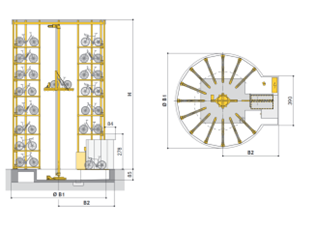
\includegraphics[width=0.5\textwidth]{images/bikesafe.png}
    \caption{Plan vom Wöhr Bikesafe \citev{woehrbikesafebroschuere}}
    \label{fig:bikesafe}
\end{figure}

\noindent Die Abbildung \ref{fig:bikesafe} zeigt die Funktionsweise vom Wöhr Bikesafe. Das System hat einen runden Aufbau, die Benutzerin oder der Benutzer gibt das Fahrrad an der Vorderseite des Turmes ab. Im Inneren des Turmes befindet sich ein Bediengerät, welches das Fahrrad zu seinem Platz bringt.
\noindent Der Nachteil des „Bikesafe“ sind die Schienen zum Einsetzen der Fahrräder. Damit ist das System nicht für alle Fahrradtypen geeignet. Außerdem ist die Lagerung von weiteren Gegenständen wie einer Jacke oder dem Helm, nicht möglich.
